\chapter{显示器的二三事}
\label{screens-and-their-secrets}

\begin{intro}
  这一章我们介绍一个\nameref{computer-and-its-components}不曾介绍过的电脑硬件——显示器。
  作为电脑与我们直接打交道的「第一线」,显示器的显示效果,直接影响着我们操作电脑的体验。
  看完这一部分,你或许能找到下面这些问题的答案:
  \begin{itemize}
    \item 为什么我的电脑屏幕看起来远没有手机 / 平板电脑那么细腻?
    \item 我喜欢画画,为什么我画出来的作品在电脑和其他设备上的颜色差距这么大?
    \item 我想选购新笔记本电脑 / 显示器,我应该关注哪些方面?
  \end{itemize}
\end{intro}

如果说眼睛是心灵的窗户,那么显示器 / 显示屏就是电脑的「心灵之窗」。
比起 CPU、内存和硬盘那些内在的配置,显示器的显示效果能够相当直观地一眼分出高低。
在这一部分,我们将介绍与显示器有关的那些事,并为大家以后选购电脑 / 显示器时提供一些参考。

\section{像素、分辨率和 PPI}

显示器上的内容是通过一个个彩色格子「拼」出来的,这样的一个小格子叫做一个「像素」或者「像素点」。
由于每个格子的颜色都可以被独立控制,我们的屏幕才得以显示各种各样的内容。

\begin{figure}[htb!]
  \centering
  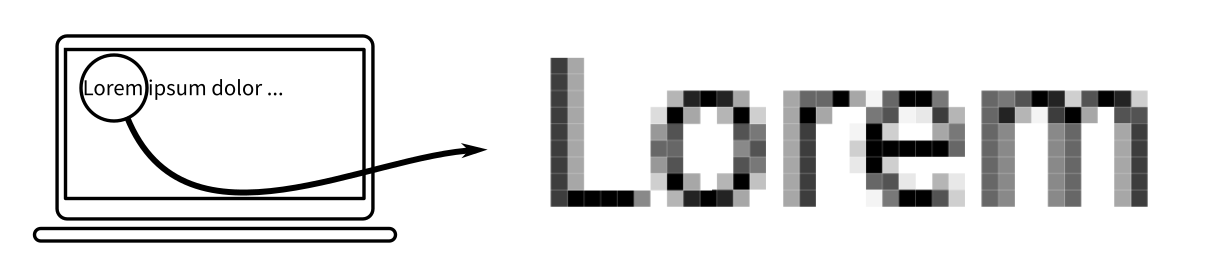
\includegraphics[width=10cm]{assets/Display.png}
  \caption{何为「显示」?}
  \label{Display}
\end{figure}

不难想象,屏幕上这样的「像素点」的个数,自然是屏幕的一个非常关键的指标。
假设现在某显示器在横向有 1920 个这样的像素点,在纵向有 1080 个这样的像素点,那么我们就把「1920 × 1080」称作是这个屏幕的「分辨率」。
顾名思义,「分辨率」影响着屏幕的「分辨」能力——分辨率越高,像素点的数量就越多,理应就有更好的「分辨」能力。

例如,假设我们有两块屏幕,它们的尺寸一样,但分辨率不同——一块屏幕分辨率高,为 1920 × 1080;
另一块低,只有 1366 × 768。如果我们让这两块屏幕显示一个同样尺寸(看起来一样大)的苹果,那么分辨率高的那块屏幕的显示效果就会更加细腻。
在屏幕尺寸相同的情况下,分辨率高的那块屏幕能拿出更多的像素点来「拼」出图像,自然「马赛克」感就要弱上许多。

\begin{figure}[htb!]
  \centering
  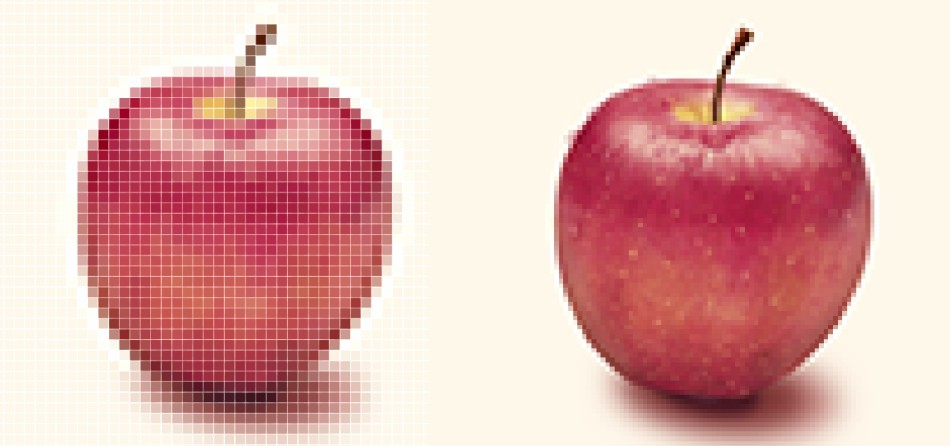
\includegraphics[width=8cm]{assets/Different_Apple.jpg}
  \caption{不同的屏幕,同样的苹果}
  \label{Different_Apple}
\end{figure}

但是,如果两块屏幕的尺寸不一样呢?假设一块屏幕分辨率高,但它尺寸也大;另一块屏幕分辨率低,可是它尺寸很小。
前者尽管有更多的像素点,可是由于屏幕尺寸变大了,像素点的「分布」依然会变得稀疏;
后者尽管像素点数量少,可是屏幕尺寸小,也许像素点看起来还更加密集呢!
这么看来,单凭一个分辨率,我们并不能直接就推断出谁的显示细腻,谁的显示粗糙。

为了公平地衡量屏幕显示的细腻程度,我们不再关注整个屏幕上的像素点的多少,而是关注屏幕在一定尺寸上像素点的多少。
具体地,我们用屏幕在 1 英寸(等于 2.54 厘米)这个长度上的像素点的个数来衡量它的显示细腻程度,这个数字称为「每英寸像素数」(pixels per inch,简称「PPI」)。
PPI 由「屏幕分辨率」和「屏幕尺寸」两个因素决定,可以通过下面这个简单的数学公式计算出来:

\[
  \mathrm{PPI} = \frac{\sqrt{w^2 + h^2}}{l},
\]

其中 $w$ 指屏幕的横向像素数,$h$ 指屏幕的纵向像素数,$l$ 是屏幕的对角线长度(以英寸计算,一般而言厂商宣传的屏幕尺寸指的就是对角线尺寸)。

现在,请你仔细观察你的电脑的屏幕和手机的屏幕。直观上,手机的屏幕要显得细腻得多——对着电脑屏幕凑近看,你或许能看出像素点之间的边界;
但对着手机屏幕,你很难再感受到那种锯齿感。
这就是因为手机屏幕的 PPI 远高于电脑屏幕造成的。
在今天,手机屏幕和电脑屏幕的分辨率相差不大,平均是在「两千上下乘以一千上下」这个水平;
但手机屏幕比电脑的小得多,PPI 因此可以达到电脑的数倍,观感自然就比电脑要好得多了。

\section{色彩和面板}

接下来,我们聊一聊屏幕的「色彩」。
屏幕的色彩体验由很多因素决定,这里我们主要介绍「色域」「色准」「色深」以及面板类型。

\subsection{色域}

首先我们简单介绍一下「色域」。
人眼能够识别的全部色彩,可以以数学和光学的方式进行一定程度的刻画。
图 \ref{CIE1931xy_blank} 展示的图形称为「CIE 1931 色彩空间」,可以理解成我们人眼能够分辨的所有颜色构成的集合。

人眼的色彩分辨能力非常强大,而以我们目前的科学技术,是造不出能够显示出所有这些颜色的显示屏的。
因此,人们在研究人眼对不同颜色的敏感程度后,从这个色彩空间中「划」出一部分子空间,用这样的子空间来指导我们生产显示器、照相机等色彩产品。
例如,图 \ref{NTSC_sRGB} 中的黑色和蓝色的两个三角形,就是两种不同的划法——一种称为「NTSC」,一种称为「sRGB」。
如果你曾经用放大镜仔细观察过电视机的屏幕,你可能会看见许许多多红、绿、蓝三色的小灯,其实这三种颜色分别就是一个显示器划出来的子区域中的三个角,也即是显示器的「三原色」。
三原色的小灯各一个才能组成一个显示器的像素,而三角形区域内所有不同的颜色都是靠这三原色以不同的明暗关系混合出来的,真是神奇啊。

\begin{figure}[htb!]
  \begin{minipage}{6.5cm}
    \centering
    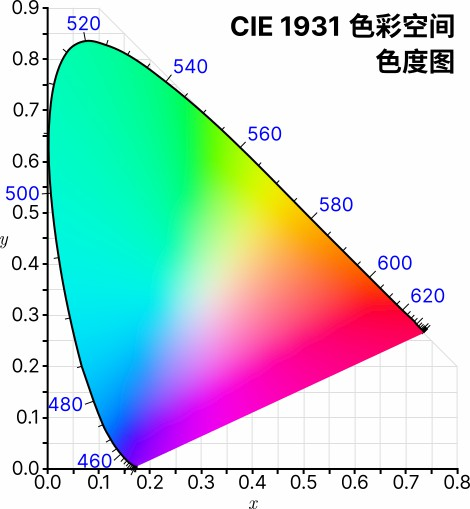
\includegraphics[width=6cm]{assets/CIE1931xy_blank.jpg}
    \caption{CIE 1931 色彩空间色度图}
    \label{CIE1931xy_blank}
  \end{minipage}
  \qquad
  \begin{minipage}{6.5cm}
  \centering
  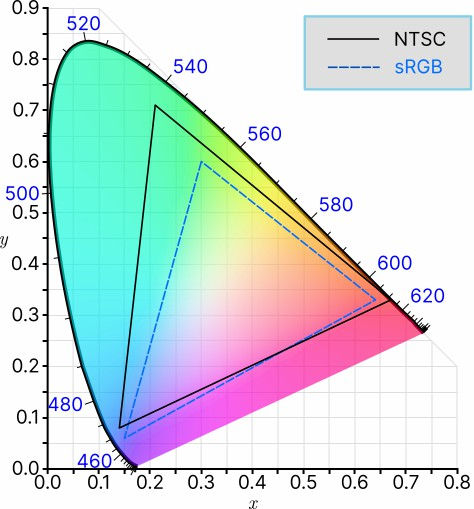
\includegraphics[width=6cm]{assets/NTSC_sRGB.jpg}
  \caption{NTSC 与 sRGB 色彩空间}
  \label{NTSC_sRGB}
  \end{minipage}
\end{figure}

然而,在这样的子空间之上,受限于成本等因素,人们发现在生产显示器时,还可以进一步「减配」——毕竟并不是所有人都要求屏幕能显示出这么多绚丽的颜色,对吧?
例如,在上面的「NTSC」色彩空间之上,再进一步划出更小的区域,用这样的小区域作为显示器色彩的标准。
例如,将 NTSC 色域的 45\% 和 72\%「拎出来」,就得到了两套更小的色彩空间:

\begin{figure}[htb!]
  \centering
  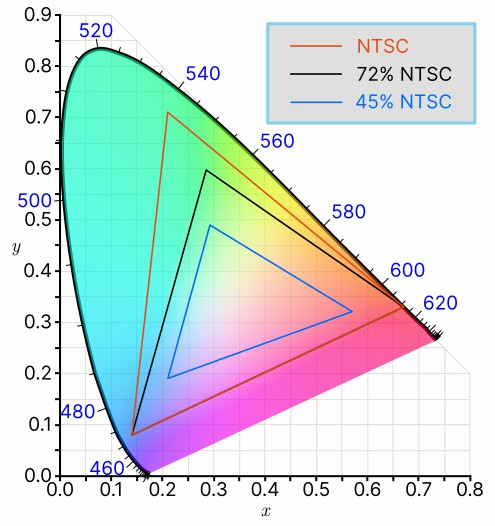
\includegraphics[width=6cm]{assets/NTSC_72_45.jpg}
  \caption{NTSC 与其子空间}
  \label{NTSC_72_45}
\end{figure}

如果某款显示器能够展现出 45\% 的 NTSC 颜色,我们就称这款显示器的「色域」是 45\% NTSC,民间有时简称 45\% 色域。
同样地,如果某显示器能展现 72\% 的 NTSC 颜色,我们就称它是 72\% 色域。
目前来说,45\% 色域又被称为是「低色域」,72\% 及以上的色域都能够统称为「高色域」。
尽管看上去 45\% 色域小得吓人,但在实际生活使用中,它也是基本足够的——除非你眼睛比较敏感,否则一眼不容易看出 45\% 色域和 72\% 色域的具体差别。
不过,如果你有进行艺术创作等的需求,或者单纯追求更舒适的体验,那么一块高色域的屏幕对你来说是非常必要的。

\begin{figure}[htb!]
  \begin{minipage}{.47\textwidth}
    \centering
    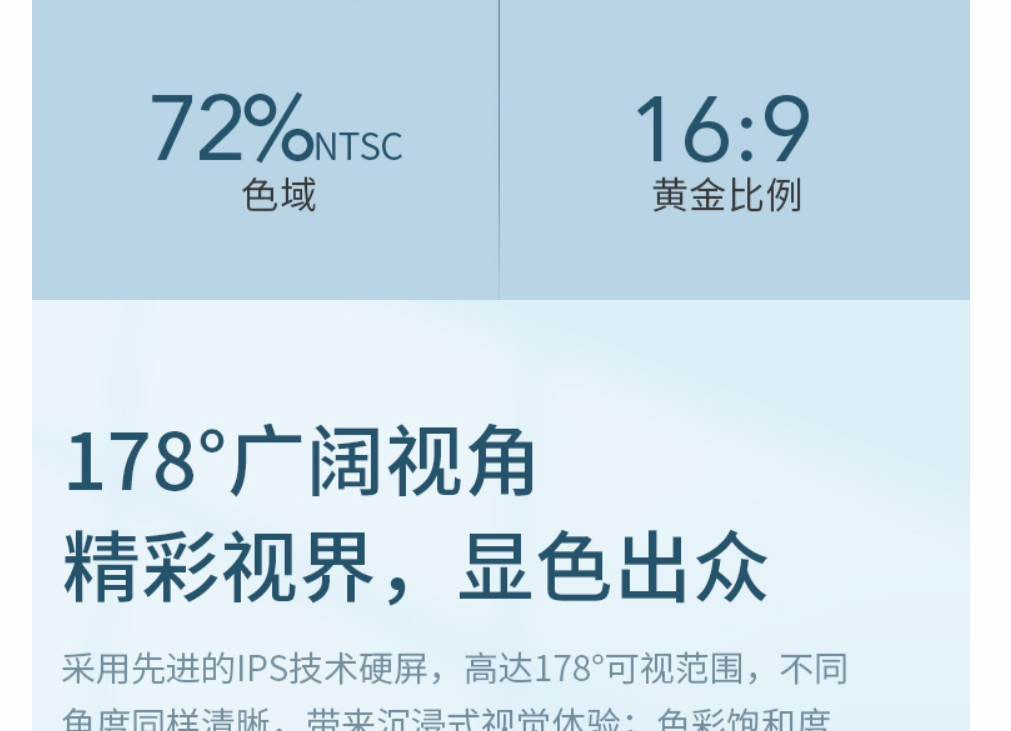
\includegraphics[width=.98\textwidth]{assets/72_NTSC_Ad.jpg}
    \caption{宣传 72\% NTSC 色域的屏幕}
    \label{72_NTSC_Ad}
  \end{minipage}
  \quad
  \begin{minipage}{.47\textwidth}
    \centering
    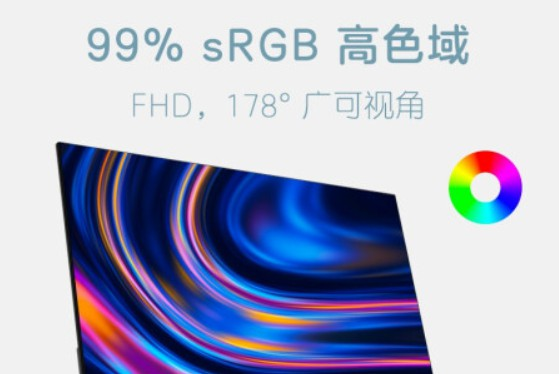
\includegraphics[width=.98\textwidth]{assets/99_sRGB_Ad.jpg}
    \caption{宣传 99\% sRGB 色域的屏幕}
    \label{99_sRGB_Ad}
  \end{minipage}
\end{figure}

除了用 NTSC 色域作为参考来「划」色域之外,现在很多厂商还会用上文中提到的另一个色彩空间 sRGB 来作为参照。
sRGB 的覆盖范围较 NTSC 小些,但它是今天使用得更普遍、更广泛的设计标准;相比之下,NTSC 则是一个老旧的电视机标准。
从色域面积上来说,sRGB 99\% 的覆盖率和 NTSC 72\% 的覆盖率基本相当,因此 sRGB 99\% 甚至更高的显示器同样是「高色域」的显示器,都能带来非常不错的体验,不过要说明的是:99\% sRGB 并不等同于 72\% NTSC。

除了 NTSC 和 sRGB 之外,还有诸如 DCI-P3 这样的更大、更专业的色彩空间,现在许多民用显示器也开始以「DCI-P3 90\%」作为自己的卖点。这里我们不再赘述相关的细节,有兴趣的读者可以自行上网查阅资料。

\begin{figure}[htb!]
  \centering
  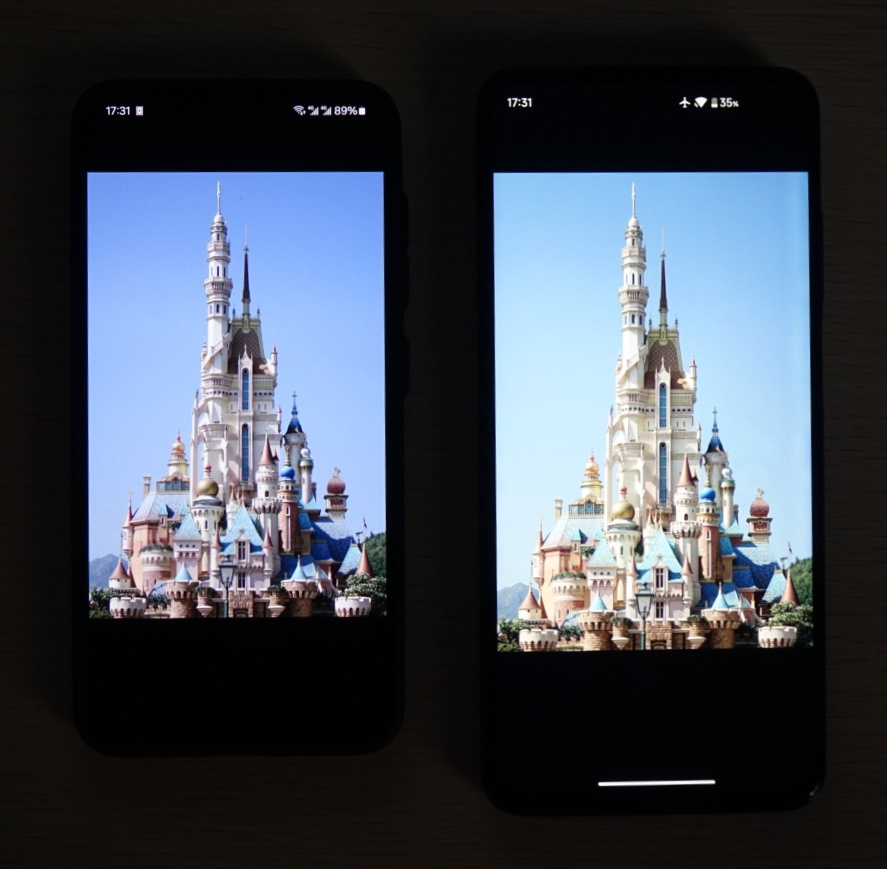
\includegraphics[width=9cm]{assets/Colour_correctness.jpeg}
  \caption{两台不同设备的色差}
  \label{Off_Color}
\end{figure}

\subsection{色准}

如果说色域决定了显示器色彩的上限,那么色准则影响着显示器的实际体验。
顾名思义,「色准」就是「色」的「准确」程度。下面是一个极端的例子:某显示器能显示 100 万种颜色,但是这 100 万种颜色的对应关系都是错的——红色会显示成绿色,蓝色会显示成紫色……那么这台显示器的体验必然是相当糟糕的。
这种色彩还原的准确程度,我们就称为一个显示器的色准。

将一张相同的图片分别在电脑、手机、平板电脑等多台设备上同时打开,再将它们并排放在一起,有时你会发现不同设备之间的色彩差异巨大。这就是「色准」的差异。
每个设备都「有着自己的想法」,对于同一个颜色的显示表现各不相同。
如果你希望自己的作品能够尽量真实地反映出颜色,那么色准将是你在选择屏幕时必须考量的因素。

色准的衡量是通过「距离」来衡量的:我们让显示器显示某个颜色 A,但显示器实际显示出来的是颜色 A*,A 和 A* 两种颜色在色彩空间图上的「距离」就能反映出这台显示器对颜色 A 的准确程度。
如果让显示器显示一系列常用的标准色,并计算各个颜色「距离」的平均值,就可以反映出一台显示器的色准水平。
具体在产品上,厂家往往用「Delta E」($\Delta E$)这个参数来描述这样的距离。
平均 Delta E 的值越小,显示器的色彩就越精准。下面是某品牌显示器的商品介绍,厂商宣称 Delta E < 2,这已经是相当高的色准了。

\begin{figure}[htb!]
  \centering
  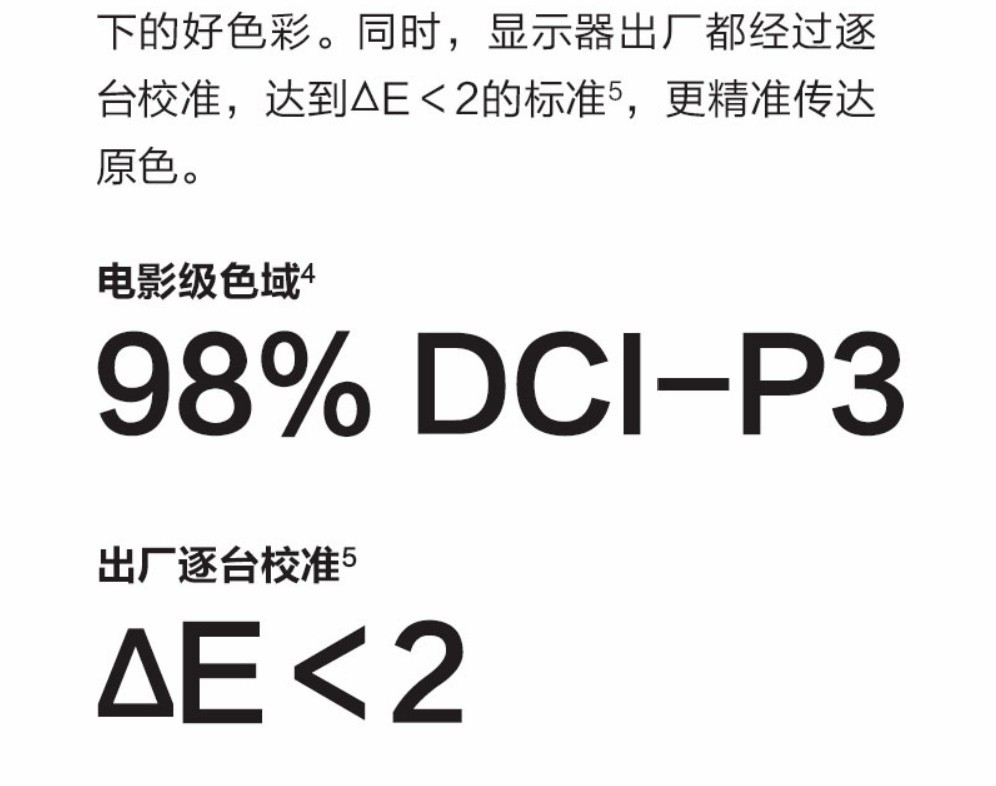
\includegraphics[width=7cm]{assets/Delta_E_below_2.jpg}
  \caption{Delta E < 2 的宣传}
  \label{Delta_E_below_2}
\end{figure}

与色域不同,色准是可以在显示器出厂后再次提升的,提升色准的过程叫做「校色」。
校色需要使用专门的设备「校色仪」,搭配专门的软件来进行。
校色的原理可以理解成重新调整显示器的显示颜色和实际颜色之间的对应关系,从而消除颜色显示的偏差。

除了购买显示器后人工校色外,一些显示器和笔记本电脑在出厂时会进行「逐台校色」,以提升显示器的出厂色准。
这也是厂商喜欢用来宣传的一个卖点。

\subsection{色深}

我们已经知道,色域决定显示画面如何绚丽,色准决定显示画面如何准确,那么「色深」则会决定显示画面如何细腻。
好的显示器,不仅能够呈现逼真而准确的色彩,更可以展示色彩细微的变化,显示器能显示的最小颜色差异即由色深决定。

衡量色深,使用的是「位深度」。
但我们先不谈「位深度」是什么,转而来看一个展示「色阶」的简单例子,假定有两台显示器的色域与色准均一致且良好,不妨以前面提到的显示器上三原色之一——红色为例,若一个红色的小灯从完全不亮(黑色)到最亮(红色)之间,显示器 A 只有 4 个层次的过渡,而显示器 B 有 8 个,那么让它们显示由黑色到红色的渐变,就会是下面这个样子:

\begin{figure}[htb!]
  \centering
  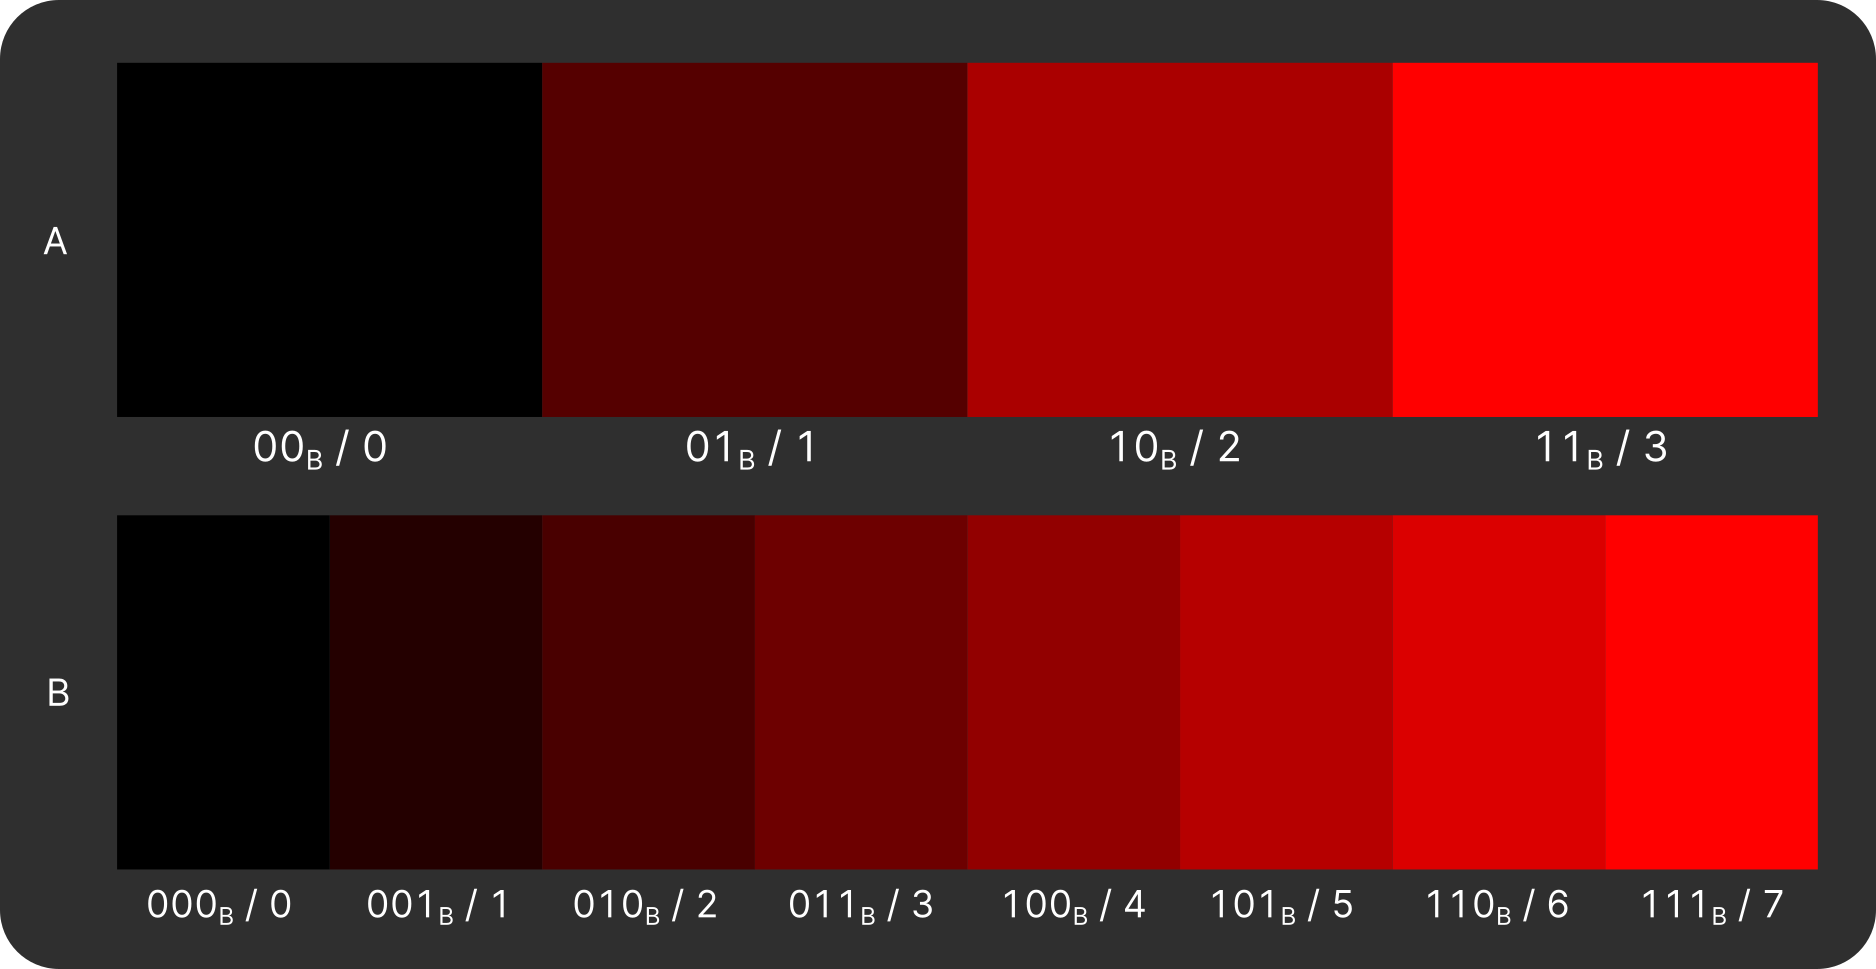
\includegraphics[width=.8\textwidth]{assets/Color_Gradient.png}
  \caption{两种色阶}
  \label{Color_Gradient}
\end{figure}

看起来 B 显示器的效果要好得多。
这些渐变的层次就是显示器能显示的色阶,上面的例子中,显示器 A 有 4 个色阶,显示器 B 则有 8 个。
如果我们分别给每个色阶指定一个数字,如图中色块底下的数值所示,来表示颜色有多「鲜艳」,那么这些值就可以被电脑用来指示显示器该如何点亮屏幕上的像素。

众所周知,计算机中的数据均是以二进制表明的,那么 $n$ 位二进制数就可以表示 $2^n$ 个不同的数值。
A 显示器有 4 个色阶,那么它只需要 2 位二进制数就能表示它拥有的所有色阶(图中带有「B」下标的数就是二进制数字);
B 显示器有 8 个色阶,所以它需要 3 位二进制数。
像这样为了表示一个显示器拥有的所有色阶所需的二进制数位数就是显示器的位深度。
需要注意的是,一般而言位深度是相对于显示器上一种颜色的小灯而言的,而不是三原色小灯加起来,但也有说法会将所有颜色的位深度加起来做宣传,譬如说 8 位的显示器「拥有 24 位色彩」,一定要仔细鉴别。

\begin{figure}[htb!]
  \centering
  
\includegraphics[width=.8\textwidth]{assets/4bit_vs_8bit.png}
  \caption{4位色深与8位色深的郁金香}
  \label{4bit_vs_8bit}
\end{figure}

很显然,位深度越大,显示器能显示的色阶越多,色彩就越细腻,图 \ref{4bit_vs_8bit} 展示了一张照片分别有 4 位与 8 位色深时的情景。
现如今,一般的显示器位深度为 8 位,也就意味着红、绿、蓝三种颜色的小灯,每一种都有 $2^8 = 256$ 种不同的亮度,所以总共可以显示 $256^3 = 16\,777\,216$ 种颜色,这也就是通常厂商宣传的「1600 万色」。
一些高端的专业显示器,色深能达到 10 位甚至 12 位,能显示的颜色也能达到 1 万亿甚至 680 万亿之巨,但对于我们普通消费者来说,10 位似乎都没有必要,所以,若没有非常专业的图像需求,普通的 8 位色深显示器就能满足日常使用了。

\subsection{面板类型}

如今的 2023 年,我们大多数人的电脑屏幕都是使用的液晶显示屏(LCD)。
液晶显示屏根据「面板类型」的不同,在观感上有着很大的差异。
目前,常见的 LCD 面板类型有 TN、IPS 和 VA 三种。
但在 LCD 之外,还存在一种称作「有机发光二极管」(OLED)的面板。
下面我们分别介绍这四种面板在色彩方面的区别。

\begin{itemize}
  \item TN 面板的显示屏(简称 TN 屏)在色彩方面表现最差。
    这种屏幕的「可视角度」非常小、而且普遍存在色彩泛白的问题。
    所谓「可视角度」小,表现在当你的视线没有正对着屏幕时,看到的颜色就有非常大的偏差。
    所谓的「色彩泛白」,可以参看图 \ref{IPS_vs_TN}。
    \begin{figure}[htb!]
      \centering
      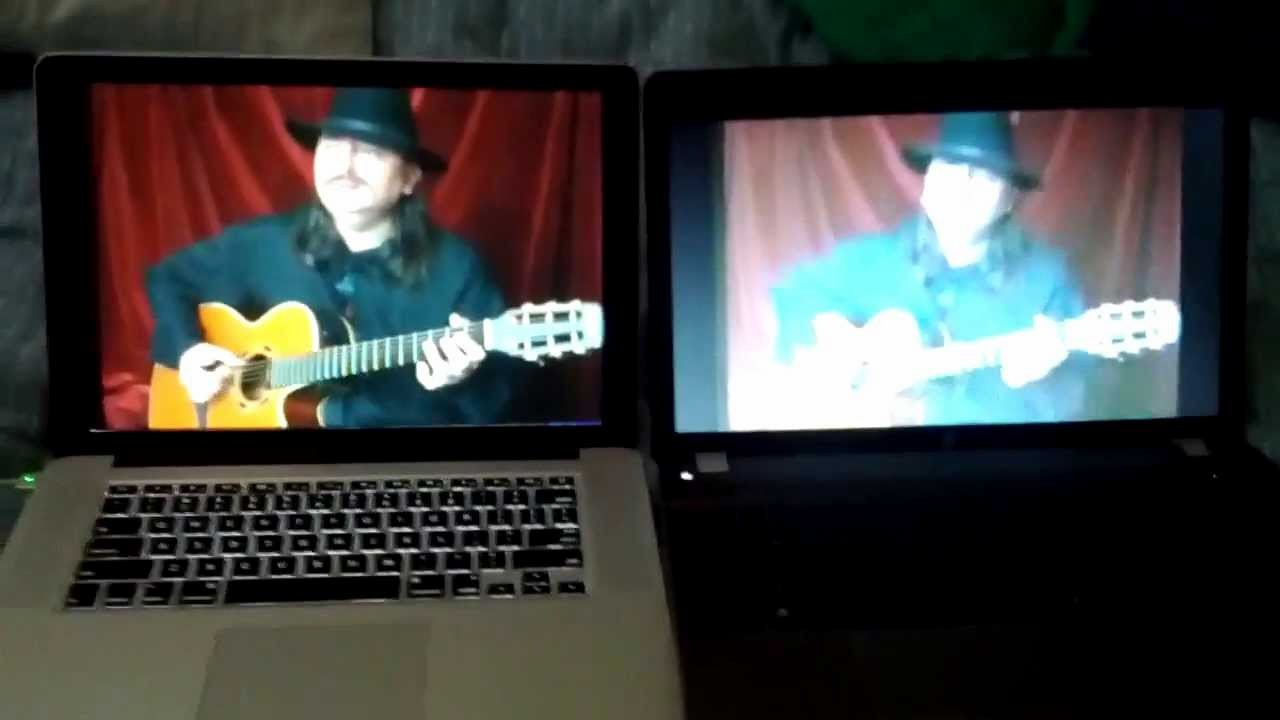
\includegraphics[width=11cm]{assets/IPS_vs_TN.jpg}
      \caption{IPS屏与TN屏的对比}
      \label{IPS_vs_TN}
    \end{figure}\\
    TN 屏是一种色域和色准都不好的屏幕。它曾经很常用,如今则主要用在低配置的显示器和笔记本上。
    尽管目前厂商也在不断改善 TN 屏的色彩,但在今天,如果你对屏幕色彩方面的观感有一定要求,那么 TN 屏都不会是你的选择。
  \item IPS 面板的显示屏(IPS 屏)在色彩方面表现相当出色。
    一方面,IPS 屏可以做到很高的色域;
    另一方面,IPS 屏有着接近于 180° 的「可视角度」——换句话说,IPS 屏无论从哪个角度看,色彩都是趋于一致的。
    这也是厂商总是会将 IPS 屏作为一个「卖点」的原因。
    在过去,IPS 屏的成本远远高于 TN 屏,因此只在高端的笔记本和显示器上使用;
    但随着科技的进步与成本的降低,IPS 屏幕几乎成为了如今笔记本与显示器的标配。
    \begin{figure}[htb!]
      \centering
      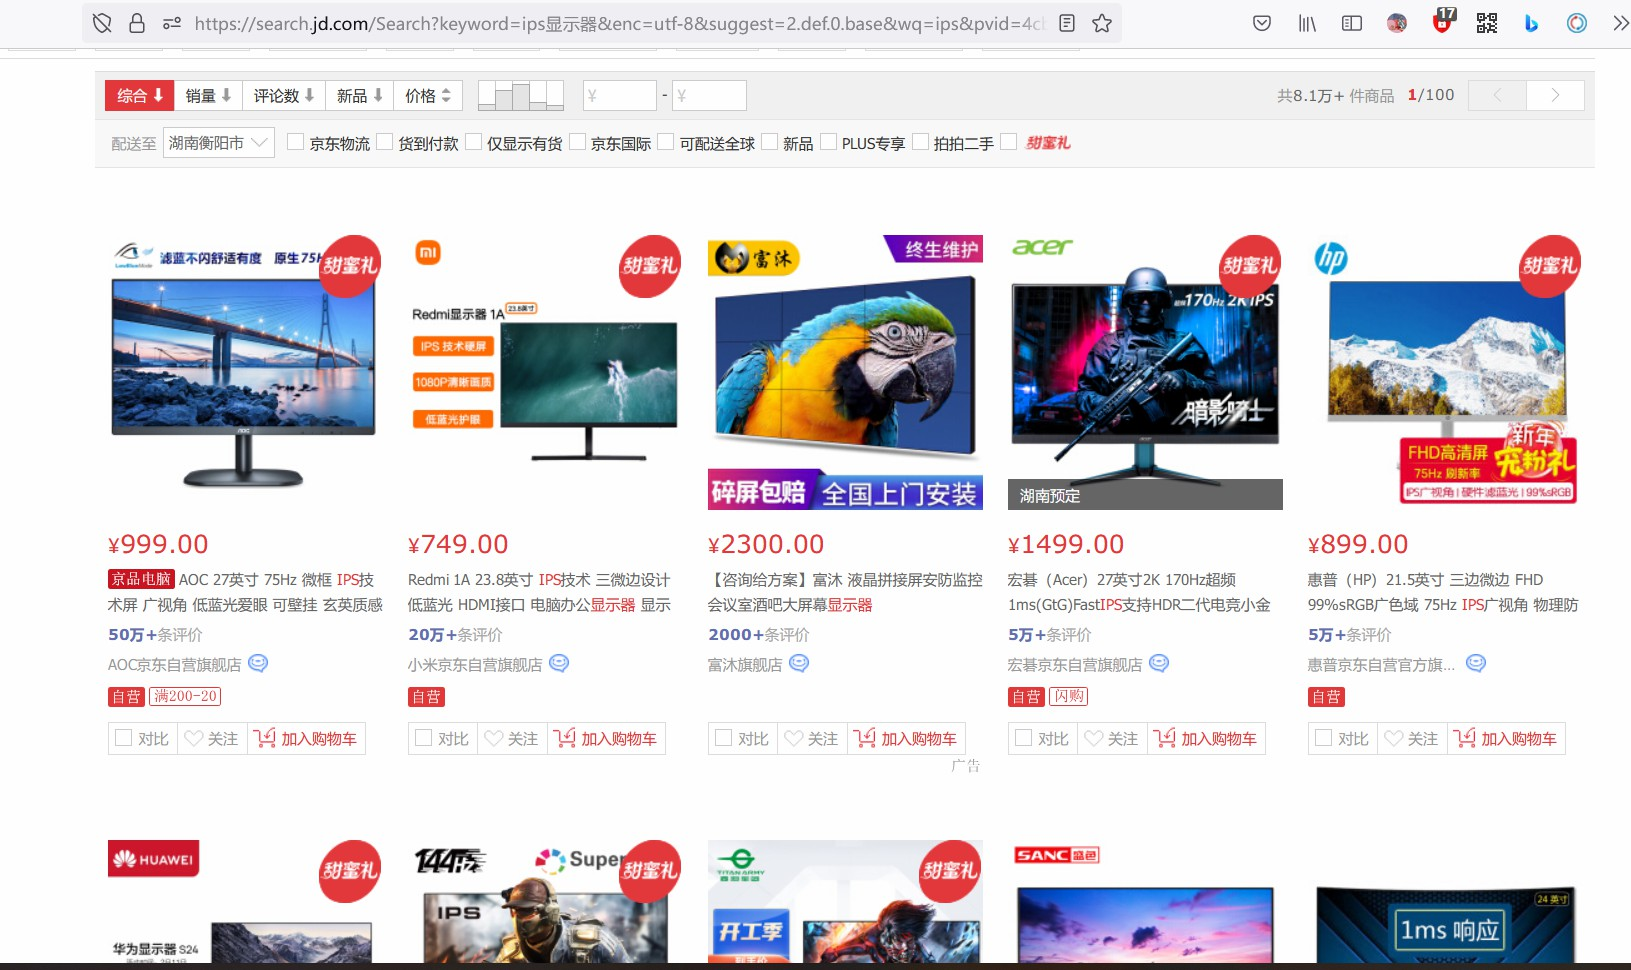
\includegraphics[width=13cm]{assets/IPS_at_Low_Price.jpg}
      \caption{市面上一些中低价位IPS屏幕}
      \label{IPS_at_Low_Price}
    \end{figure}\\
    当然,同样是 IPS 屏幕,它们仍然有色域和色准的区别。
    换言之,我们的比较必须是多维度的:总体上,IPS 屏幕的观感好于 TN 屏幕;
    高色域的 IPS 屏幕的观感好于低色域的 IPS 屏幕;色准好的 IPS 屏幕观感好于色准差的屏幕。
  \item VA 面板的显示屏(VA 屏)也是一种色彩相当优秀的屏幕。
    VA 屏由于技术上更容易做大、做宽,而且还可以做成曲面,同时价格没有 IPS 那么高,因此市面上的很多低价「带鱼屏」「曲面屏」都在使用 VA 面板。
    VA 面板的缺点主要是拖影比较严重,因此在某些程度上不是十分适合游戏。
    下图是某品牌千元级的「带鱼屏」产品,使用的就是 VA 面板。
    \begin{figure}[htb!]
      \centering
      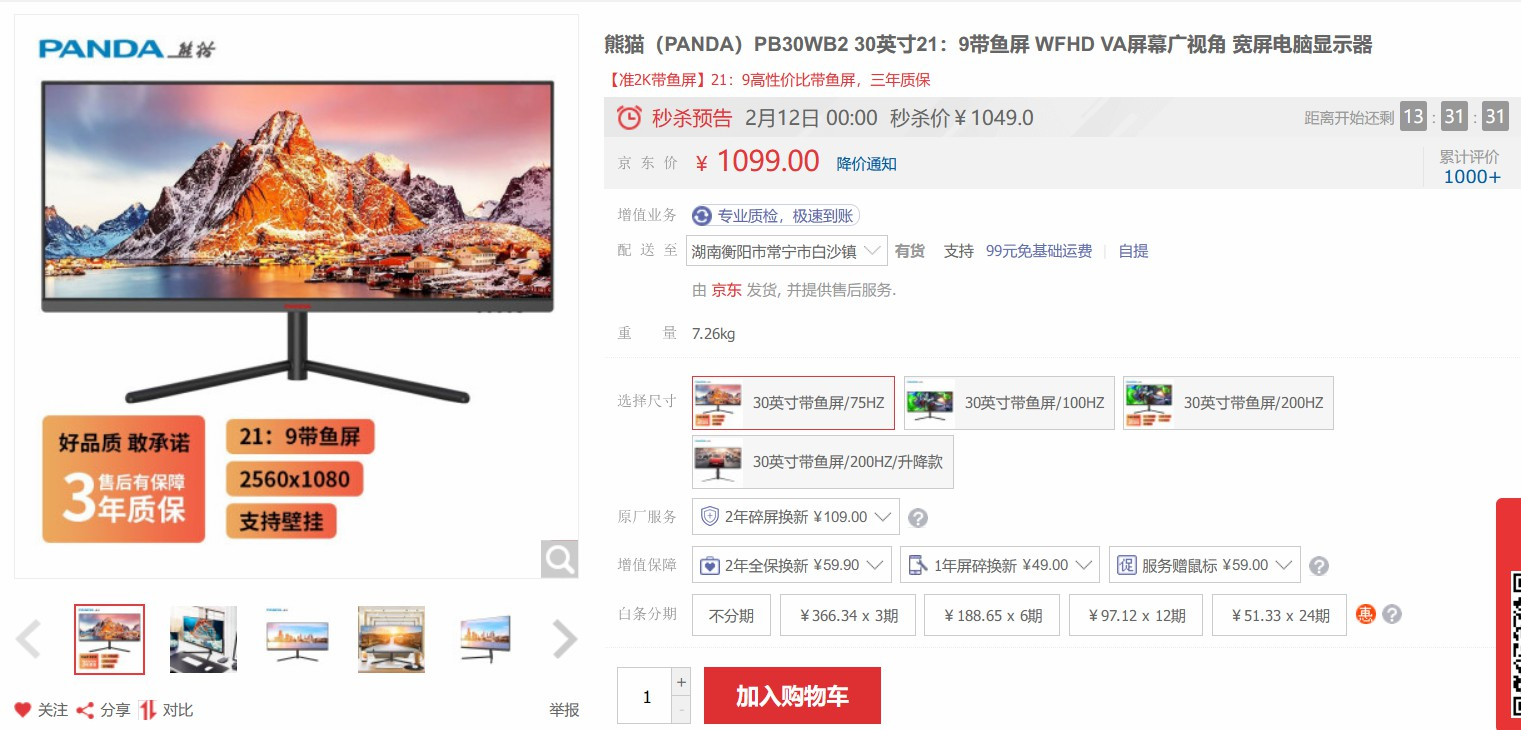
\includegraphics[width=11cm]{assets/VA_at_Low_Price.jpg}
      \caption{千元VA「带鱼屏」}
      \label{VA_at_Low_Price}
    \end{figure}\\
    VA 面板是一种色彩优秀的高性价比选择。
    如果你不怎么玩游戏,但又喜欢「大屏」「宽屏」「曲面屏」,那么一众 VA 屏可能就是你的意中「屏」。
  \item OLED 屏幕是近年来市场上的一种新兴屏幕面板类型,带来了与之前所言的几种 LCD 面板完全不同的体验。
    LCD 与 OLED 的显示原理大致如下图所示,可见 LCD 依靠背板发光、液晶偏转、颜色滤光来显示出不同亮度与不同颜色,而 OLED 依靠不同颜色的二极管自发光来显示。
    这种原理上的根本区别使得 OLED 拥有高亮度、高对比度、更薄、响应更迅速、颜色更艳丽的优势,但由于 OLED 自身材料的局限性,它也有着成本较高、寿命短、烧屏(即屏幕留下永久残留影像)等缺点。
    \begin{figure}[htb!]
      \centering
      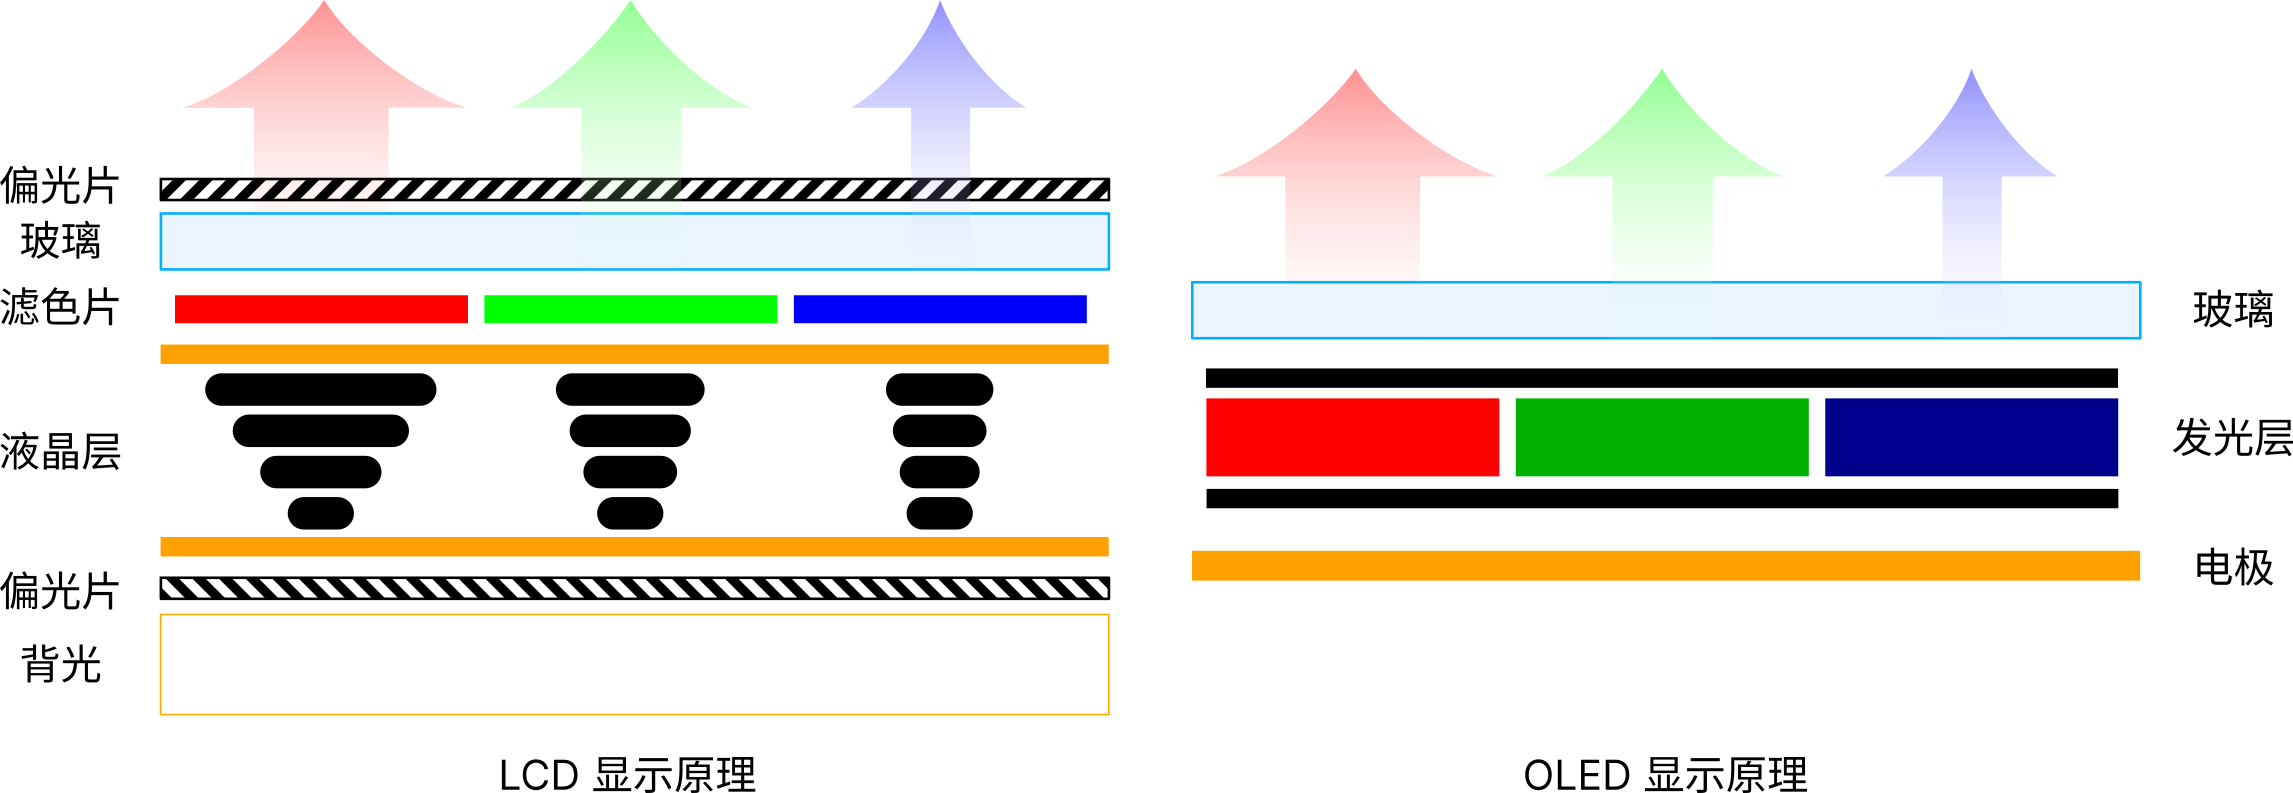
\includegraphics[width=.8\textwidth]{assets/LCD_OLED.png}
      \caption{LCD与OLED的显示原理}
      \label{LCD_OLED}
    \end{figure}\\
    除此之外,OLED 的一大优势是柔软,甚至可以折叠起来。
    不难发现,如今新款手机的显示屏一般是 OLED 面板,而且很多带有一些弧度,而低端机型仍然在使用 LCD。
    下图就是同一张图片在使用 LCD 面板与 OLED 面板的手机上的显示效果(均为最高亮度),可见 OLED 的色彩层次更丰富,而 LCD 的一大缺点就是「黑色不黑」,这是背光无法完全被遮住导致的。
    但在低亮度下,一些 OLED 的亮度调节策略是「频闪」(即 PWM 调光,在「开关开关」的循环中利用开、关时间之比来模拟低亮度),使得它容易导致眼睛疲劳,影响健康。
    \CJKsout*{所以说关灯睡觉了就不要在床上玩手机了。}
    \begin{figure}[htb!]
      \centering
      \includegraphics[width=.8\textwidth]{assets/LCD_OLED_Phone.jpg}
      \caption{LCD与OLED的显示效果}
      \label{LCD_OLED_Phone}
    \end{figure}\\
    近两年,许多笔记本电脑与显示器也开始配备 OLED 面板,但占有的市场份额并不大,普遍而言价格要高于同尺寸与分辨率的 IPS LCD 屏幕,一般在 2000 元以上。
    但另一方面,由于 OLED 的颜色与亮度优势,高色深的显示器更容易制造出来,然而价格也在普通 OLED 显示器上更进一步。
    所以,如果你想追求更好的色彩效果,同时预算充足,可以考虑 OLED 显示器。
\end{itemize}

\section{刷新率}

也许你已经知道,显示器是利用人眼的视觉暂留效应,将一张张的静态画面「拼」成动态画面并展示给我们看的。
然而,显示器不可能做到「拼」的速度无限快,每秒钟换几十张已经是很多显示器的极限。
这个「每秒钟换几十张」就是显示器的刷新率,它的单位是赫兹(Hz)。
例如,60 Hz 的显示器,它每秒钟最多能向我们展示 60 幅画面;而 120 Hz 的显示器,则每秒可以展示 120 幅。

\begin{figure}[htb!]
  \centering
  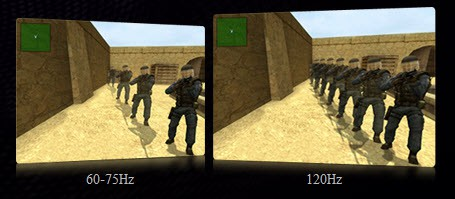
\includegraphics[width=8cm]{assets/60Hz_vs_120Hz.jpg}
  \caption{不同刷新率的对比}
  \label{60Hz_vs_120Hz}
\end{figure}

如果你是游戏玩家,那你自然会知道「帧率」这个概念。
帧率是电脑每秒可以生成的画面的数目,而刷新率是显示器每秒能够显示的画面的个数。
最理想的情况下,帧率和刷新率相等,这样电脑生成的每一幅画面都能完美地被显示器展现。
如果帧率很高,但刷新率不够,那么就会有许多幅画面没能够被显示——显示器跟不上画面来的速度;
如果帧率低,而刷新率高,那么显示器就会在多次显示同一帧。
这两种情况都会造成一个恶性后果:画面有「撕裂」感。
诸如「垂直同步」「FreeSync」之类的选项可以避免这两种情况带来的画面撕裂,具体细节请读者自行上网查找。

在今天,大多数办公用的笔记本和显示器的刷新率都是 60 Hz 或 75 Hz。
一些游戏本和游戏显示器的刷新率则能达到 120 Hz、144 Hz 甚至更高。
更高的刷新率能带来更流畅的游戏体验(前提是,你的配置足够好,能够到达这么高的帧率),但也意味着更高的价格。
如果你是游戏玩家,那么这将是你需要考虑和进行取舍的一个因素。

\section{总结}

在文章的最后,我们为大家总结一下选购显示器时的关注点:

\begin{enumerate}
  \item 分辨率和尺寸:想要更加「细腻」的显示效果,\regcolor{在尺寸相同的条件下选分辨率高的}。
    比如,13 寸的笔记本屏幕,分辨率最好在 1920 × 1080 以上;21 寸的台式机显示器,分辨率最好在 2560 × 1440 以上。
  \item 色域与色准:若对色彩有要求,\regcolor{选择「DCI-P3 90\%」「100\% sRGB」「99\% sRGB」「72\% NTSC」等高色域}的显示器;
    对色准有要求,选择厂商\regcolor{宣称「出厂校色」并且 Delta E 比较小}(例如,Delta E < 2)的显示器。
  \item 色深:\regcolor{日常使用则选择 8 位显示器},但若有图像处理等专业需求,选择色深 10 位及以上的显示器。
  \item 面板类型:\regcolor{选择 IPS 屏幕或者 VA 屏幕。}
    TN 屏非常「瞎眼」,除非你知道自己在做什么,否则不要选择。
  \item 刷新率:若你\regcolor{追求游戏性能,在配置(尤其是显卡)足够的情况下,选择 144 Hz、120 Hz 等高刷新率}的;
    反之,60 Hz、75 Hz 和 90 Hz 的显示器已经足够满足你的需求。
\end{enumerate}

\practice

\begin{enumerate}
  \item 查看你电脑显示器的分辨率。可以通过在桌面上右键 →【显示设置】→【显示分辨率】来查看。
  \item 了解你电脑显示器的尺寸。尺寸指的是屏幕对角线的长度,一般单位是「英寸」(inch)。然后,结合上一题查到的分辨率,计算你屏幕的 PPI。
  \item 查找你电脑显示器的色深。可以去桌面上右键 →【显示设置】→【高级显示器设置】找找。
  \item 在电商平台上查找显示器 / 笔记本电脑,看看厂商有没有宣传屏幕的色域、色准和刷新率信息。
\end{enumerate}